\chapter{Materials and Methods}
\label{02methods}

\colorbox{yellow}{Materials and methods. For the main thesis chapters presenting method development work, the methods section below will contain the more technical methodological information, while the results chapters will focus more on the implementation of the tool or method.

REMEMBER TO BE CONSISTENT WITH TOOLS/PACKAGES/FUNCTIONS styles}.

\newpage

\section{CyGNAL}

\begin{wrapfigure}[26]{l}{0.45\textwidth}
    \vspace{-.5cm}
    % \centering
    \definecolor{foldercolor}{RGB}{124,166,198}
    \tikzset{pics/folder/.style={code={%
        \node[inner sep=0pt, minimum size=#1](-foldericon){};
        \node[folder style, inner sep=0pt, minimum width=0.3*#1, minimum height=0.6*#1, above right, xshift=0.05*#1] at (-foldericon.west){};
        \node[folder style, inner sep=0pt, minimum size=#1] at (-foldericon.center){};}
        },
        pics/folder/.default={20pt},
        folder style/.style={draw=foldercolor!80!black,top color=foldercolor!40,bottom color=foldercolor}
    }
    \forestset{is file/.style={edge path'/.expanded={%
            ([xshift=\forestregister{folder indent}]!u.parent anchor) |- (.child anchor)},
            inner sep=1pt},
        this folder size/.style={edge path'/.expanded={%
            ([xshift=\forestregister{folder indent}]!u.parent anchor) |- (.child anchor) pic[solid]{folder=#1}}, inner xsep=0.6*#1}, %change to ysep/xsep for horizontal
        folder tree indent/.style={before computing xy={l=#1}},
        folder icons/.style={folder, this folder size=#1, folder tree indent=3*#1},
        folder icons/.default={12pt},
    }
    \frame{
        \begin{forest}
            for tree={font=\sffamily, grow'=0, %comment out grow=0 for horizontal
            folder indent=.9em, folder icons,
            edge=densely dotted}
            [CyGNAL Main Folder
                [Analysis%, this folder size=20pt
                    [Step\emph{N}\_input]
                    % [..., is file]
                    [Step\emph{N}\_ouput]
                    % [..., is file]
                    [Vis\_Step\emph{N}]
                ]
                [Preprocessed\_Data
                ]
                [Raw\_Data
                    [5 Sample FCS files, is file]
                ]
                [Utils\_Data
                ]
                [code, this folder size=20pt
                    [aux]
                        % [Auxiliary modules with functions, is file]
                    [utils]
                        % [Optional steps and misc. utilities, is file]
                    [\texttt{1-data\_preprocess}, is file]
                    [\texttt{2-umap}, is file]
                    [\texttt{3-emd}, is file]
                    [\texttt{4-dremi}, is file]
                    [\texttt{5v1-htmp}, is file]
                    [\texttt{5v2-pca}, is file]
                ]
                [docs]
                [figs]
                [\texttt{conda\_env.yml}, is file]
                [\texttt{dependency\_troubleshoot}, is file]
            ]
        \end{forest}
    }
    \begin{spacing}{1}
    \caption{Directory Structure of \newline CyGNAL.}
    \end{spacing}
    \label{fig:cygnal_dir}
\end{wrapfigure}

Written mainly in Python and R, CyGNAL (CyTOF SiGNalling AnaLysis) is a pipeline constituted as a series of core scripts within the \texttt{code} directory. Considered as the main steps of CyGNAL, these scripts have been numbered according to the canonical order within CyGNAL's workflow. The first script handles data preprocessing and must always be run. The second script embeds cells in a two-dimensional UMAP \colorbox{yellow}{[or PHATE]} space. The third and fourth steps compute the EMD and DREMI scores, which can then be visualised using either Heatmaps in step \texttt{5v1} or as through PCA in step \texttt{5v2}.

Python modules containing function definitions are kept within the \texttt{aux} directory, while the \texttt{utils} directory contains optional steps and utility scripts for data handling. The resulting modular structure allows for general utility functions used throughout CyGNAL to be defined once within a single file. 
Data ingestion and egestion is done through a series of input and output directories, either specific to each of the main steps or common for all scripts within the utilities folder.


\newpage

\subsection{Deployment and dependencies}

CyGNAL is intended to be deployed as a non-standardised pipeline by cloning the directory to a local machine. However, to minimise any possible dependency issues, CyGNAL includes a Conda environment \texttt{YML} file. Conda \colorbox{yellow}{ADD REF} is a package and environment management system that works with multiple programming languages, including Python and R. Hence, with the included \texttt{YML} file, a software environment with all of CyGNAL's R and Python dependencies might be replicated in a single step.

% \fcolorbox{yellow}{FUTURE WORK}While ideally a framework like \emph{nextflow}\colorbox{yellow}{ADD REF/LINK} would be used

However, there are cases when the Conda environment fails to solve and a suitable environment can not be generated, such as when using different compute architecture. For these instances I have also prepared a containerised distribution method using Docker \colorbox{yellow}{ADD REF}. Based on an x86 Debian Linux container, CyGNAL's container automates the process of creating a Conda environment with all required dependencies on platforms with a different architecture like ARM-based Apple Sillicon.

This container is hosted on Docker Hub and can be \emph{pulled} from \texttt{docker.io/ferranc96/cygnal:one}.

Running CyGNAL from the Docker container only requires of two additional steps:

\begin{itemize}

\item Pull CyGNAL from the GitHub repository, place it in your home directory (i.e. \texttt{\textasciitilde}), and rename the \emph{CyGNAL} folder to \emph{CyGNAL\_docker}. 

\item Run the following command on the host terminal:\newline
\texttt{docker run -v \textasciitilde/CyGNAL\_docker/:/usr/app/CyGNAL -it\newline
--entrypoint /bin/bash -p 12241-12252:12241-12252\newline
docker.io/ferranc96/cygnal:one}. 

\item Use CyGNAL commands on the container terminal as described in the relevant chapter \colorbox{yellow}{ADD REF}

\end{itemize}

The docker command above runs a live terminal on the container with a Conda environment that already contains all necessary dependencies. Communication with the host machine is done via the shared directory in \texttt{~/CyGNAL\_docker} (i.e. where you will need to input data and fetch CyGNAL's outputs), with open ports to access the Heatmap and PCA shinyApps. 
It is important to note that on first run it will take some time to pull the image (~1.5GB), and that alternative container tools such as Podman \colorbox{yellow}{ADD REF} should work but are not officially supported.

Furthermore, should the user encounter any issues while using CyGNAL, the Python script \texttt{dependency\_troubleshoot.py} should help locate and report to the user any missing dependencies.

\subsection{Computation}

During the pre-processing step CyGNAL loads in mass cytometry files either as tab-separated plain text format or in the Flow Cytometry Standard (FCS) format (FCS)\cite{spidlen_data_2010}. Intercompatibility between both formats is ensured using the Python packages \emph{fcsparser}\cite{yurtsev_eyurtsevfcsparser_2020} and \emph{fcswrite}\cite{noauthor_zellmechanik-dresdenfcswrite_2021}, and the R package \emph{flowCore}\cite{ellis_flowcore_2021}. In addition to ensuring format consistency and allowing for datasets to be saved in either format, during the pre-processing step channel names are parsed to; a) eliminate empty channels; b) clean up double spaces and underscores; and c) ensure each cell has a unique ID encoded in a new column called “Cell\_Index”. This is accomplished using the \texttt{rename\_columns} and \texttt{filter\_columns} functions via regular expressions (Table \ref{tab:cygnal_regex}).

\begin{table}[h!]
\centering
\begin{tabular}{| p{3cm} p{3cm} p{6.4cm} |} 
    \hline
    \textbf{Function} & \textbf{Main Regex} & \textbf{Description} \\ [0.5ex] 
    \hline\hline
    \texttt{rename\_columns} & 
    \begin{tabular}[t]{@{}c@{}}
    \verb/(__[a-z].*$|/ \\ \verb/__\d.*$|/ \\ \verb/_\(.*$|/ \\ \verb/___.*$)/
    \end{tabular} &
    % \begin{minipage}[t]{0.4\columnwidth}
        Expression catches badly formatted channel names with doubled or tripled underscores, so that the function can simplify channel names.
        % matches a string that starts with one of the following:
        % \begin{itemize}\setlength\itemsep{0em}
        %     \item Two underscores followed by a lowercase letter and any number of characters until the end of the line.
        %     \item Two underscores followed by a digit and any number of characters until the end of the line.
        %     \item One underscore followed by an opening parenthesis and any number of characters until the end of the line.
        %     \item Three underscores followed by any number of characters until the end of the line.
        % \end{itemize}
    % \end{minipage} 
    \\
    \hline
    \texttt{filter\_columns} & 
    \verb/^\d+[A-Za-z]+$/ & 
    % \begin{minipage}[t]{0.4\columnwidth}
        pattern that matches a string that starts with one or more digits followed by one or more letters until the end of the line.
    % \end{minipage} 
    \\ [1ex] %adds extra space
\hline
\end{tabular}
\caption{Table to test captions and labels.}
\label{tab:cygnal_regex}
\end{table}

Finally, this first preprocessing step also writes to disk a panel\_markers.csv file containing those columns present in the dataset that were identified as markers (i.e. where the channel name is composed of an isotope and an antibody or other cellular marker. The panel\_markers.csv file can then be used by the user to filter out certain channels for downstream steps.

CyGNAL’s Universal Manifold Approximation and Projection (UMAP) calculation uses the \emph{umap-learn} package \cite{mcinnes_umap_2020} to embed the cells in a 2-dimensional space. The embedding is computed using the set of markers defined by the user in the panel\_markers.csv file and can be calculated on either just one processed dataset or a series of datasets as long as they have shared markers in their panel. The resulting coordinates are appended as a new pair of columns to the original datasets, facilitating visualisation of this space elsewhere by the user.

EMD stands for Earth Mover's Distance and is named so because it can be intuitively thought of as the amount of work required to transform between two piles of earth, where work refers to the mass of earth to be moved times the distance. Also known as the 1\textsuperscript{st} Wasserstein distance (\(W_1\)), we define it between two 1D arrays of measured values \(u\) and \(v\) as:
\[W_1(u, v) = \int_{-\infty}^{+\infty} |U-V|\]
Where \(U\) and \(V\) are the cumulative distribution functions of \(u\) and \(v\) respectively.

Applied to the mass cytometry datasets in CyGNAL, we score each marker (chosen via the panel\_markers.csv file) based on its distribution of intensities in a variable dataset (\(u\)) when compared to a particular reference (\(v\), either defined from the sum of all datasets imputed or a particular dataset selected by the user). The absolute value of the distance metric is then signed based on the median values of the variable and reference distributions in order to assign a direction to the changes observed that can then be interpreted in a biological setting (e.g we want know how much the apoptotic marker cCaspase 3 [D175] changes between a condition and the control, but also where its median intensities are higher).

Described in Van Djik et al. 2018 \cite{van_dijk_recovering_2018}, \emph{k}-NN conditional Density Resampled Estimate of Mutual Information (DREMI) is a mutual information metric that reflects how informative the distribution of intensities for marker A is in describing the intensities of maker B (i.e. \(I(A|B)\) ). Unlike the EMD scores that compares across conditions then, DREMI is computed on a per condition basis, where each of the possible combinations of markers in panel\_markers.csv is scored.

Both the EMD and DREMI scores are computed using the Python package \emph{scprep} \cite{noauthor_krishnaswamylabscprep_2021}, and the outputs of both scoring systems are saved as plain text files that can be plotted using CyGNAL’s visualisation steps below.

It is important to note that for calculating the EMD and DREMI scores and computing the UMAP space, the data is by default normalised using an inverse hyperbolic \(asinh x\) transform with a co-factor of \(5\). However, the user is prompted to override the default behaviour if so desired, and the co-factor value can be easily changed within the various scripts.

\subsection{Visualisation}

\colorbox{yellow}{This reads more like it should be in the main chapter}

CyGNAL  automates and allows for the user to visualise both EMD and DREMI scores in an interactive manner via Shinny-Apps\cite{noauthor_rstudioshiny_2021}. 

The Shiny-Apps are contained within R files loaded from the last main scripts of the CyGNAL workflow. For this, user defined arguments in the python scripts need to be parsed to the R Shiny server when it is called through bash using Rscript.

The first of the visualisation scripts generates a series of heatmaps using the \emph{ggplot}\cite{wickham_ggplot2_2009} and \emph{ComplexHeatmap}\cite{gu_complexheatmap_2021} packages. These heatmaps show the relevant scores; with the names of the datasets used in the calculation step as columns in the horizontal axis and the names of the markers in the vertical axis as rows. Colour ranges, columns, and rows shown can all be tweaked by the user through the graphical interface. 
The second of the scripts computes a PCA on the scores using the \emph{FactoMineR} package\cite{le_factominer_2008}, treating each of the datasets used in the calculation as observations and the scores for the markers (or marker pairs in the case of DREMI) as variables. In all cases, all plots generated can be saved as images for later use, and within the PCA Shiny-App the computed PCA coordinates can also be downloaded to facilitate custom generation of plots elsewhere.

% \subsection{Submodules}
% Second part of this could go into the main body of results chapter
% Within the aux directory are contained several python scripts with functions imported during the usage of CyGNAL. The resulting modular structure allows for general utility functions used throughout CyGNAL to be defined once within a single file. 


\section{Cell State Random Forest Classifier}

The cell state classifier built uses the \emph{scikit-learn} Python package \cite{pedregosa_scikit-learn_2011} to train a Random Forest classification algorithm and assign cell state labels to mass cytometry datasets. A Random Forest (RF) algorithm is based on a series of decision trees, simple non-parametric models that predict the class of an observation by learning decision rules inferred from the data during training. By using a randomised collection of these trees (i.e., a forest) the RF palliates the tendency of decision trees towards overfitting while at the same time reducing the variance of the results. \colorbox{yellow}{Give more info on this} This is so because each of the individual trees sees only a subset of the data, hence they built different models. Then, being an ensemble method, when each datapoint is passed through them all, a majority vote decides on the class given.

Hosted in \url{https://github.com/FerranC96/C\_StateML}, this Cell-State RF classifier consists of two Python scripts and shared auxiliary functions. 
The first of the scripts is used to train a model from labelled data and report on its performance against validation and testing datasets. Default parameters are used for the Random Forest (except for an increase in the number of decision trees to 480), and the cell state classes in the training data are balanced by donwsampling to the least common state. Pre-trained models are also included in the repository as will be detailed below.
Balancing classes is done to ensure that all cell states are trained using the same number of cells and so that performance metrics such as $F_1$ scores, which are vulnerable to imbalanced classes, can be used.

The second script is used to run a saved RF model through new mass cytometry datasets to label and assign a state to each cell. While designed to work with unlabelled data, if the input data is already labelled this script also reports on the model's performance. 

Performance evaluation is reported both as text and in the form of plots, and consists of; 1) confusion matrices, 2) log losses, 3) precision, recall, and $F_1$ scores for each class. 

 For class $c$, let:
\[precision_c = \frac{TP_c}{PredP_c}\]
where precision is also known as Positive Predictive Value, $TP_c$ is the number of true positives, and $PredP_c$ the number of predicted members in $c$,

and let
\[recall_c = \frac{TP_c}{P_c}\]
where recall is also know as True Positive Rate and $P_c$ is the number of cells in $c$,

the $F_1$ scores for each class $c$ are defined as the harmonic mean of the precision and recall of $c$ so that:
\[F_1 = 2 \frac{precision \cdot recall}{precision + recall}\]

Before both training and evaluation the data is assumed to be in the form of raw intensities and gets transformed using an inverse hyperbolic \(asinh x\) transform with a co-factor of \(5\). 

\begin{figure}
    \centering
    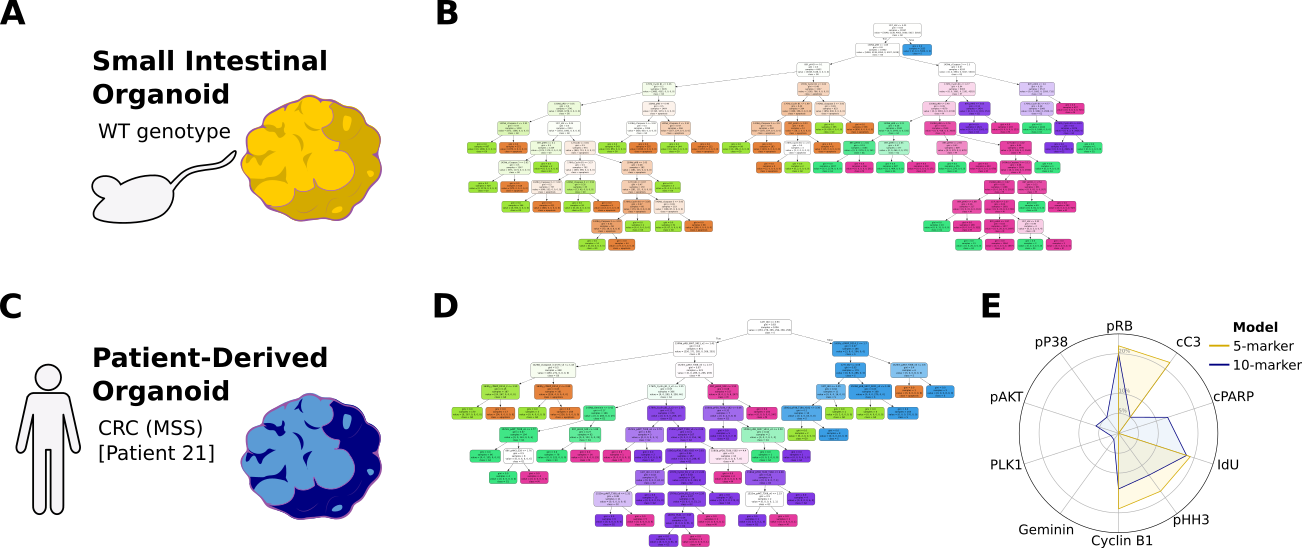
\includegraphics{02methods/figs/2CYTOF_trainRFclass.png}
    \caption{}
    \label{}
\end{figure}

This classifier implementation was used to build two models distinguished by the features they use and the type of epithelial cells they were trained on. 

The simpler 5-marker model uses only 5 cell state markers and was trained using a balanced subset of cells from the Small Intestinal murine organoid time-course experiment in Qin et al. 2020 \cite{qin_cell-type-specific_2020}. This model uses the same exact antibody markers as those used by Qin et al. 2020 to label cell state via manual gates, namely: pRB [S807/S811], cleaved Caspase 3 [D175], IdU, Cyclin B1, and pHH3 [S28].

The more complex 10-marker model was trained using CRC Patient Derived Organoids. With an updated panel, the markers used in the latest models are a set of ten antibodies (the five markers from above plus cPARP [D214], pAKT [T308], pP38 [T180/Y182], Geminin, and PLK1) with targets specific to each of the six cell state classes (Apoptosis, G0, G1, S-phase, G2, and M-phase). The data used to train this model has been published in Ramos Zapatero et al. 2023 \cite{zapatero_trellis_2023} and belongs to an untreated monoculture replicate of PDO21. 

Details on the markers used in the RF models, and the cell state they are associated with, can be found in \colorbox{yellow}{Table XXXXX} \ref{tab:markers}. 

\begin{table}[h!]
\centering
\begin{tabular}{| p{3.6cm} p{4.8cm} p{3.6cm} |}
    \hline
    \textbf{Marker} & \textbf{Specificity} & \textbf{Model} \\
    \hline\hline
    pRB [S807, S811] & Proliferating cells & 5-marker, 10-marker \\
    \hline
    pAKT [T308] & PTM in the mTOR pathway (proliferation) & 10-marker \\
    \hline
    pP38 [T180, Y182] & PTM promoting \textbeta-cat activation (proliferation) & 10-marker \\
    \hline
    pHH3 [S28] & M-phase & 5-marker, 10-marker \\
    \hline
    PLK1 & G2/M-phase transition & 10-marker \\
    \hline
    Cyclin B1 & G2 & 5-marker, 10-marker \\
    \hline
    IdU & S-phase & 5-marker, 10-marker \\
    \hline
    Geminin & Negative marker of G1. Expressed in S-phase, G2, and M-phase & 10-marker \\
    \hline
    cCaspase 3 [D175] & Apoptosis & 5-marker, 10-marker \\
    \hline
    cPARP [D214] & Apoptosis & 10-marker \\
    \hline
\end{tabular}
\caption{Table of Markers}
\label{tab:markers}
\end{table}

    % Some of the results presented in this document correspond to an initial implementation of the RF algorithm that used only 5 different cell state markers: pRB [S807/S811], cleaved Caspase 3 [D175], IdU, Cyclin B1, and pHH3 [S28]. This 5-marker implementation was trained using a balanced subset of cells from SI LGR5 time-course experiment in Qin et al. 2020 \cite{qin_cell-type-specific_2020} (downsampled so that all six cell states would have the same number of cells, 5306). The trained model was then tested against datasets from the same publication; a simpler single-timepoint SI LGR5 culture, and a complex coculture of colonic organoids (with varying degrees of CRC mutations and TME complexity).
    % In contrast, the latest results use data acquired from Patient Derived Organoids of CRC patients. With an updated panel, the markers used in the latest models are a set of ten antibodies (the five markers from above plus cPARP [D214], pAKT [T308], pP38 [T180/Y182], Geminin, and PLK1) with targets specific to each of the six cell state classes (Apoptosis, G0, G1, S-phase, G2, and M-phase). This 10-marker model was trained on an untreated control condition replicate and testing is performed against a second set of replicates comprising a total of 5 conditions (plus an untreated control) treated with increasing concentration of the chemotherapeutic topoisomerase inhibitor SN-38.


    % \colorbox{yellow}{TRain a model and evaluate performance}
    % The script performs the following tasks:
    
    % Imports necessary libraries and modules.
    % Sets up input/output directories and creates necessary folders if they don't exist.
    % Asks for user input to provide information about the run.
    % Checks if the specified output directory already exists and exits the script if the run name has been used before.
    % Reads and processes the training data from a specified directory.
    % Balances the classes in the training data by downsampling if necessary.
    % Translates antibody markers in the training data.
    % Prepares the training and validation datasets for the random forest classifier.
    % Trains a random forest classifier and performs calibration on it.
    % Generates predictions and probabilities for the test data using the trained model.
    % Evaluates the performance of the model using various metrics such as classification reports, confusion matrices, and log loss.
    % Saves the trained model and outputs relevant plots and reports.
    
    % \colorbox{yellow}{Classify a dataset using a pre-trained model}
    % The script performs the following tasks:
    
    % Importing necessary libraries and modules: pandas, numpy, matplotlib.pyplot, os, sys, joblib, sklearn, and seaborn.
    % Importing custom functions from the "aux" module.
    % Setting up the folder structure for input and output data.
    % Defining the model to use for labeling cell states and loading the corresponding model file using joblib.
    % Prompting the user to provide information about the run and handling the input.
    % Checking if the input data is already labeled with cell states.
    % Reading the input data from the specified folder and storing it in a list.
    % Checking the features used in the model and translating the column names of the input data to match those features.
    % Handling data preprocessing steps such as filtering and normalizing.
    % Predicting cell states on the input data using the loaded model.
    % Adding the predicted labels to the original data frames and saving the results as CSV files.
    % Calculating and displaying prediction scores (accuracy, balanced accuracy, classification report, confusion matrix, F1 score) if the input data is labeled.
    % Saving the classification report and confusion matrix as files and plotting the confusion matrix.



\section{scRNA-seq Data Analysis}

Work presented in this section has already been made public in Qin \& Cardoso Rodriguez et al. 2023 \cite{cardoso_rodriguez_single-cell_2023}. As a joint co-first authored paper, attribution is shared between Dr. Xiao Qin and myself. While I carried out all of the scRNA-seq Data Analysis presented in this Thesis, Dr. Xiao Qin was in charge of the murine colonic organoid culture system and data acquisition via both scRNA-seq and Mass Cytometry. The exact attribution for specific tasks is detailed in Qin \& Cardoso Rodriguez et al. 2023 \cite{cardoso_rodriguez_single-cell_2023}. 

Aiming to provide additional context, the section below on scRNA-seq data acquisition has been included despite Dr. Xiao Qin having carried-out the work.

% \subsection*{Wet Lab Data Generation}

% This work wasn't carried out by me and this should be made very clear. Instead of detailing it here, perhaps it would be best to reference the preprint/article once up?

% Generation of murine colonic organoid heterocellular cultures as shown in 


\subsection*{scRNA-seq Data Acquisition}

In brief, the organoid heterocellular culture system was dissociated into single-cells, FAC-Sorted for live cells, counted and fixed with methanol before scRNA-seq library preparation. For co-cultures, different cell-types were mixed at equal cell numbers prior to the fixation step. scRNA-seq libraries were generated with the 10X Genomics Chromium Next GEM Single Cell 3' Reagent Kits v3.1 (Dual Index) and sequenced with the Illumina NovaSeq 6000 System (2$\times$ 150 bp paired-end reads), aiming at 60,000 read pairs per cell and 2,000 cells per cell-type per sample.

\subsection*{Data Processing}
% Raw scRNA-seq data was converted to FASTQ files and processed with the 10X Genomics Cell Ranger pipeline version 5.0.1. Sequencing reads were aligned to a custom GRCm38 reference genome containing the sequences of \hl{\textit{DsRed} and \textit{eGFP}} transgenes present in fibroblasts and organoids respectively.

The Illumina NovaSeq binary base call (BCL) outuput sequence files were converted to FASTQ files and processed with the 10X Genomics Cell Ranger pipeline version 5.0.1 \cite{10x_genomics_what_nodate}, which provides with a convenient wrapper for Illumina's bcl2fastq tool \cite{illumina_bcl2fastq_nodate}, \texttt{cellranger mkfastq}. Prior to alignment, a custom murine GRCm38-based reference genome was generated using the STAR aligner \cite{dobin_star_2013} wrapper \texttt{cellranger mkref}. By adding the sequences for \textit{DsRed} and \textit{eGFP} transgenes present in fibroblasts and organoids respectively, cell type discrimination based on exogenous transcripts was facilitated. Then, alignment of the FASTQ files against this custom reference was performed using the \texttt{cellranger count} pipeline, generating both unfiltered and pre-filtered feature-barcode matrices.

The resulting feature-barcode matrices were analysed with the R package \textit{Seurat} version 4.0.4 \cite{hao_integrated_2021}. 
The analysis pipeline encompasses quality control, data normalisation, data integration, dimensionality reduction, cell clustering, and analysis of differential gene expression. 
Genes found in less than 4 cells were removed during QC and only cells with at least 600 unique genes identified were kept for downstream analysis. The total number of detected reads per cell typically ranged from 1,200 to 80,000, with the actual values manually determined based on dataset sequencing depth and cell-type composition. 
Cell type composition was considered as the macrophages were observed to be captured less efficiently than fibroblast or epithelial cells.
For the integrated epithelial object in used throughout the analysis, an additional filtering step was performed to remove cells with undetectable expression for any one of the \emph{bona fide} pan-epithelial genes \textit{Epcam}, \textit{Krt8}, \textit{Krt18}, \textit{Krt19}, \textit{Cldn7}. 
Doublet/multiplet filtering was explored using the scDblFinder package \cite{germain_scdblfinder}, which has been designed to find heterotypic doublets such as those that could be present in co-culture conditions. However, after the QC pipeline outlined above, the low number and homogeneous distribution on 2D embeddings of the putative doublets was not deemed convincing enough to warrant their removal.

The Seurat object, much like its SCE counterparts in R or AnnData objects in Python, contains multiple layers where different barcode x feature matrices can be stored. This is so it can accommodate for different normalisation methods and for tools that expect raw or processed gene expression values. 

Gene expression values were normalised for total counts, multiplied by a scale factor of  \(1\cdot10^4\), and the expression values log transformed as \(X = \log_2 (X+1)\). The resulting normalised count matrix was used for methods that rely on the explicit comparison or visualisation of gene expression.

An alternative normalisation approach was used as described in Hafemeister \& Satija 2019 \cite{hafemeister_normalization_2019}. Named sctransform (SCT) this method models both biological and technical variation using the Pearson residuals from a regularised negative bionamial regression. The nature of this model allows for certain signals to be regressed out, such as the percentage of mitochondrial transcripts over the total reads in a cell, or for differences between cycling cells in different phase of the cell cycle. We computed SCT normalised count matrices with 6,000 features and regressed out mithoncondrial content and differences between cell cycle phases.

Cell Cycle scores were computed using the CellCycleScoring function from Seurat (a wrapper for AddModuleScore) and a curated list of cell cycle genes shown in \ref{appendix:cycle}. By comparing how well a cell matches the G2 and M-phase signature, versus a G1 and S-phase signature, cells could be classed into Dividing cells (Mitosis and G2), Cycling (G1 and Synthesis), and Other (cells with low scores for both signatures, most likely outside of the cell cycle). Differences between the Dividing and Cycling groups were also regressed out when computing the SCT normalised count expression data, as it was deemed that intra-cycle differences were not central to the biological system being studied. \colorbox{yellow}{ADD REF TO APPENDIX}

Throughout the study, steps that relied on building a k-NN graph or low-dimensional representation of the data use either the SCT normalised data or the SCT-derived integrated representation (see section below).

\subsection*{Integration}

Dataset integration was performed using Seurat's reciprocal PCA (RPCA) implementation \cite{hao_integrated_2021} as it has been optimised to handle large datasets. RPCA works by projecting the individual datasets into an other's PCA space to identify cellular anchors with shared neighbourhoods across projections. The integration itself is described in Stuart et al. 2019 \cite{stuart_integrative_2019}, so that new expression matrices in the integrated space are computed based on the difference of expression matrices between anchor cells. Inherently a pairwise process, integration of multiple datasets is done iteratively by pairs accordings to their pairwise distances. In this work I used the SCT normalised data as the feature space to be integrated and ran default parameters but for a k.anchor of 12.
The integrated object presented in \colorbox{yellow}{XXX} was computed using all cells from the 20 conditions shown in Figure \colorbox{yellow}{XXX}, resulting in a total of 58,726 cells with the integrated assay limited to 2,000 genes. The integrated object presented in Figure \colorbox{yellow}{XXX} was computed using just the epithelial cells from all conditions, resulting in an object with 29,452 cells limited to 4,000 genes. The respective integrated feature spaces were stored within the integrated assay of the Seurat object.

The integration pipeline with anchors found via Canonical Correlation Analysis was also tested, but as described in the literature, it was found to be less computationally efficient and appeared to smooth out and erase too much biological signal \cite{stuart_integrative_2019}. \colorbox{yellow}{(small figure comparing umap from cca VS rpca, coloured by crctme label)}.

When handling the aggregated data from multiple CRC patient cohorts presented in Joanito et al. 2022 \cite{joanito_single-cell_2022}, where data integration was performed mostly for visualisation purposes, the methods described above struggled to handle the high number of cells present (>40,000 cells). As one of the goals of this data integration approach was to compare our murine organoids with human samples, I used scVI \cite{lopez_deep_2018}, a Variational AutoEncoder approach that can be GPU-accelerated and performs well on inter-species integration tasks \cite{song_benchmarking_2023}. Part of a broader family of PyTorch-based methods for analysing single-cell omics data \cite{gayoso_python_2022}, scVI learns a low dimensional latent space that can be used to compute 2-dimensional embeddings of the data. Able to account for multiple quantitative and categorical confounding variables, this method can also handle the projection of query datasets onto an integrated reference.
Cross-species data integration was thus achieved by generating an integrated reference from the human CRC datasets and projecting into it a humanised version of the mouse organoid data described earlier in this work \colorbox{yellow}{(batch effect as XXXX)}. The integrated human reference was built using unique patient identifiers as the batch key and controlling for the percentage of mitochondrial reads in a cell. The resulting latent space was embedded into 30 dimensions. Humanisation of the mouse count matrix was accomplished via the mousipy package \cite{peidli_mousipy_2023}, which facilitates the handling of mouse genes with multiple human orthologues.
Untransformed data was used for the scVI workflow \colorbox{yellow}{(validate this statement!)}. 

\subsection*{Dimensionality Reduction}

To generate the EMD PCA plots shown in Figure \colorbox{yellow}{XXXXX} I used the normalised gene expression data of all cells of a particular cell type (organoids, fibroblasts, or macrophages) stored within the RNA assay of the integrated Seurat object from \colorbox{yellow}{XXX}. EMD scores for the top 6,000 variable genes of each condition were computed with CyGNAL \cite{ferran_cardoso_tape-labcygnal_2021} using the relevant control condition for each cell type: WT monoculture for epithelial organoids, fibroblast monoculture for fibroblast cells, and macrophage monoculture for macrophage cells. The collection of gene-specific EMD scores for each condition was then used to compute a PCA space where each dot represent a whole condition.

The standard pipeline for generating single-cell embeddings consisted of computing a set of 50 to 100 principal components (PC) from a normalised count matrix, from which 2-dimensional PHATE embeddings were generated with default parameters \colorbox{yellow}{(see Table S\ref{})}. PHATE was chosen as the default DR method for visualisation due to its capacity to capture the global structure in biological settings with important developmental trajectories \cite{moon_visualizing_2019}. In the context of integrated datasets via scVI, the 30-dimensional latent space was used to generate the PHATE embeddings. 
This mid-dimensional PCA space was also used to compute most of the \emph{k}-NN cell-cell graphs used throughout the study. 


\subsection*{Unsupervised Clustering and Differential Expression}

Cell clustering was computed using the Leiden algorithm on the \emph{k}-NN graph generated from the integrated epithelial dataset (first 48 PCs), at a series of resolutions ranging from 0.2 to 0.8. The final cluster annotations were retrospectively defined by common cell-type marker expression, inter-cluster relationships on a multi-resolution clustering tree \cite{zappia_clustering_2018}, and cross-condition differential abundance behaviours (see below). Cells from outlier clusters (totalling less than 1\% of all epithelial cells) were excluded from the downstream analysis. \colorbox{yellow}{REF THE FIGS WHERE THE CLUSTS ARE SHOWN}.

Differentially Expressed (DE) genes between clusters, conditions, and cell neighbourhoods were identified using Wilcoxon rank-sum tests as implemented in Seurat's \textit{FindAllMarkers} and \textit{FindMarkers} functions. The Wilcoxon rank-sum test is commonly used in the field of scRNA-seq as it.... Non parametric, assumption being that samples being compared are independent. DE results in the form of log transformed Fold Changes in gene expression and p-values adjusted for multiplicity of tests.

Heatmaps of selected marker genes were generated with the R package \textit{ComplexHeatmap} \cite{gu_complex_2016}. Gene lists in \colorbox{yellow}{UPDATE:Figures \ref{fig:fig1}I and Figure \ref{suppfig:figs1}B} were curated from previously reported markers for colonic epithelial subpopulations and DE genes detected between epithelial clusters, conditions, and DA neighbourhoods within this study. Gene lists in \colorbox{yellow}{\ref{suppfig:figs1}B-D} represent DE genes between conditions.

\subsection*{Differential Abundance}

Differentially abundant (DA) cell neighbourhoods were identified using the R package \textit{MiloR} \cite{dann_differential_2022}. Milo works by constructing cellular neighbourhoods on a \emph{k}-NN graph. These neighbourhoods can overlap with one another, for cells may belong to multiple neighbourhoods at once, and act as the basis of Milo's compositional analysis. By comparing the composition of these neighbourhoods in terms of a categorical variable of interest (condition), Milo assigns them an enrichment score (log Fold Change) according to the relative abundace of cells from the query or control condition. Significance and regression out of technical and unwanted biological variables is achieved though a Generalised Linear Model via the mature edgeR package \cite{robinson_edger_2010}, and using the SpatialFDR metric (first described in Lun et al. 2017 \cite{lun_testing_2017}).
DA analysis thus allows for the detection of enrichment and depletion of epithelial cell states caused by microenvironmental and/or genotypical perturbations in the organoid system. 

For the analysis shown in \colorbox{yellow}{FIGURE NUMBER} I set the DA test threshold at 5\% SpatialFDR (Figure \ref{fig:fig1}F). In the context of fibroblast regulation of the colonic epithelia, given that CD34\textsuperscript{hi} and CD34\textsuperscript{lo} fibroblasts do not differentially regulate epithelial cells \colorbox{yellow}{(Figure \ref{suppfig:figs1}B)}, all samples of WT organoid+fibroblast co-cultures were grouped and considered replicates of the query condition regardless of the CD34 status of the fibroblasts. AK and AKP organoid monocultures were also grouped due to their similar DE and DA behaviour (Figure \ref{fig:fig1}G).
The DA overview dot plot in Figure \ref{fig:fig1}H was generated by comparing the 17 conditions against the WT monoculture control (2$\times$ replicates). Size of the dots represents the number of neighbourhoods associated with a particular combination of cluster and conditions, while dot colour shows the median log Fold Change value for those neighbourhoods. Absence of replicates in this approach results in a lack of relevance for the SpatialFDR statistic, and the control condition (1st row) was populated with empty values for visualisation purposes. 

The \emph{k}-NN graphs used by Milo where constructed as detailed in the section above.

\subsection*{Signature score correlations}

The \textit{UCell} \cite{andreatta_ucell_2021} method was used to generate the correlation matrix between gene signatures in existing literature and cell clusters identified within this study \colorbox{yellow}{(Figure \ref{suppfig:figs2}A)}. UCell uses the Wilcoxon rank-sum test, also known as Mann-Whitney U, and a matrix of ranked genes (by expression) for each cell in the dataset. Given a list of genes, UCell can then score how well each cell matches their expression. Unlike Seurat's AddModuleScore function (and it's re-implementaion in scanpy), the resulting scores are not normalised against a control gene set, making UCell scores impervious to dataset composition. 

Gene lists for different intestinal stem cell-states were compiled from public datasets, together with transcriptional targets of key signalling pathways encoding the different stem cell-states \colorbox{yellow}{NEED TO MAKE THIS TABLE}. Gene identifiers where transformed to murine Gene Symbols (to be compared with the features in the sequencing dataset) by querying BioMart \cite{smedley_biomart_2009}. These gene lists were compared with the curated gene signatures for proliferation, CSC, revCSC, and proCSC cell-states in \colorbox{yellow}{Figure \ref{fig:fig1}I}, as well as the top DE genes for each stem cluster (adjusted p-value < 0.01, log2FC > 0.25, top 24 genes with the greatest positive log2FC values) \colorbox{yellow}{(Table S3)}. \textit{UCell} scores for each gene set were calculated using Log-normalised gene expression values and z-scored to allow cross-signature comparison.

\colorbox{yellow}{EMBED TABLE HERE}
\ref{tab:SignMD}
By gathering more than 50 gene lists from the literature \colorbox{yellow}{POINT TO GITHUB OR TO SUP TABLE} that describe key signalling pathways and stem-related gut epithelia states, I could put the results of this study in context with a broader corpus of works in varied settings, such as human data, cancer, or tissue repair.

Pearson correlations were computed between the relevant scores (i.e. those whose context refers to the stem compartment or key signalling pathways) on all cells of stem and TA clusters and then visualised as a heatmap-like correlation matrix with the corrplot package \cite{wei_r_2021}. Signatures that did not have a SD deviation of scores greater than 0.2 across the cells where excluded from the analysis (as they would equally mark all states present in the dataset), and matrix entries where populated for significant correlations (confidence level of 0.95, )heatmap entries were only showing significant correlations (conf.level = 0.95, based on Pearson's product moment correlation coefficient). Finally, the matrix was ordered and grouped via complete linkage hierarchical clustering (k=3). 



\subsection*{Signalling Entropy}

Leveraging the concept that cells with a higher potency should have a higher signalling entropy \cite{teschendorff_signalling_2014}, the pluripotency values for epithelial cells across the different clusters were estimated using the R package \textit{SCENT} \cite{teschendorff_singlecell_2017}. 
Signalling entropy scores for all epithelial cells in \colorbox{yellow}{INT EPI OBJECT FIGURE} were determined via the CCAT approximation method, which computes a Pearson correlation between a cell's transcriptome and the interactome as defined by the built-in \textit{net17Jan16} Protein-Protein interaction network (derived from the Pathway Commons database). As the interaction network is annotated with NCBI gene IDs, BioMart was used to translate them to MGI gene symbols.

Being a method that is completely independent of any cell metadata, like clusters or conditions, the resulting vector of CCAT scores was added as a new metadata column to the sequencing dataset object and used to compare pluripotency in \colorbox{yellow}{VIOLIN PLOTS} and as one of the components of the Valley-Ridge score \colorbox{yellow}{REFE TO VR SECTION!(\ref{})}


\subsection*{RNA Velocity}

For RNA velocity analysis, loom files were generated from Cell Ranger's output using the command line interface tool \textit{velocyto} \cite{lamanno_rna_2018}. The murine GRCm38 reference was used, with the GRCm38/mm10 repeat mask assembly and the RepeatMasker track. RNA velocity was analysed with the Python package \textit{scVelo} \cite{bergen_generalizing_2020} using default parameters unless otherwise specified \colorbox{yellow}{(Table S2)}. Metadata and PHATE embedding coordinates were exported from the relevant Seurat objects to filter and annotate AnnData objects generated from the loom files made by velocyto. Moments for the velocity estimation were calculated using the first 50 PCs and 30 neighbours from the AnnData objects. RNA velocities were computed with the \textit{recover\_dynamics} function using the dynamical model of transcriptional dynamics with default parameters. The velocity stream embedding (Figure \ref{fig:fig1}E) was computed using the integrated object containing epithelial cells from all conditions. The RNA velocity vector lengths, an estimate of a cell's rate of transcriptional change, were computed using cells solely from the 4 conditions shown in Figure \ref{suppfig:figs2}B-D. The quantitative comparison in Figure \ref{suppfig:figs2}D was performed using the Games-Howell pairwise test wrapper from the R package \textit{statsExpressions} \cite{patil_statsexpressions_2021}. All conditions were compared against the WT monoculture control and all \textit{p}-values have been corrected for multiplicity with the Holm method.

Initial and terminal macrostates where determined using CellRank \cite{lange_cellrank_2022}, which leverages RNA velocity information to describe cellular dynamics. The matrix of cell-cell transition probabilities was constructed as a weighted combination of the transition matrix based on velocity directions (through the VelocityKernel class, weight of 0.8) and a symmetric transcriptional similarity matrix (through the ConnectivityKernel class, weight of 0.2). Macrostates, and their transition probabilities, were computed using the built-in Generalised Perron Cluster-Cluster Analysis (GPCA) estimator. To find initial macrostates, inverse velocity vectors are used to assemble the transition matrix by setting the backward argument to \texttt{True} when computing the VelocityKernel component. 

\subsection{Cell-to-cell communication analysis}

Cell-cell communication inference was performed using the R package CellChat \cite{jin_inference_2021}, where stromal-epithelial signalling was analysed across 4 different organoid genotypes (WT, A, AK, and AKP).
CellChat uses a database of interactions between ligands, receptors, and cofactors \cite{noauthor_cellchatdb_nodate}. Using cluster annotations and the gene expression matrix, interaction probabilities can be inferred between the different populations using a permutation-based approach. The inferred interactions can the be grouped at the pathway level, and functional analysis of the clusters can be infered via network analysis methods. 

Epithelial cells were annotated with the clusters previously identified \colorbox{yellow}{(Figure \ref{fig:fig1}D)}, while the fibroblasts were grouped as a single cluster. A merged CellChat object was generated to compare relative communication probability of fibroblast-to-epithelia signalling across the genotypes. Significant ligand-receptor pairs were identified based on CellChat's murine cell communication database. Plots displaying aggregate outgoing and incoming communication probability \colorbox{yellow}{(Figure \ref{fig:fig4}A)} were generated with the \textit{netAnalysis\_signalingRole\_scatter} function. Detected communication at the pathway and interaction level was accessed with the \textit{subsetCommunication} function and probabilities were z-score normalised to allow for cross-pathway or cross-interaction comparison. The results were visualised with ComplexHeatmap in \colorbox{yellow}{Figure \ref{fig:fig4}B-C}, the rows of which were manually ordered based on hierarchical clustering and grouped based on the nature of the interaction. Gene expression of the ligand-receptor pairs identified above was visualised using Seurat's \textit{Dotplot} function in Figure \ref{suppfig:figs5}A. \textit{UCell} scores for ligand and receptor genes were calculated for fibroblasts and epithelial cells respectively. Games-Howell pairwise test was performed using the R package \textit{statsExpressions} and all \textit{p}-values have been corrected for multiplicity with the Holm method.



\section{VR score and data-driven Waddington-like landscapes}

Work presented in this section has already been made public in Qin \& Cardoso Rodriguez et al. 2023 \cite{cardoso_rodriguez_single-cell_2023}. While I am the author behind the Valley-Ridge (VR) score design and implementation, including the python-based renders of the data-driven Waddington-like landscapes. 

Dr. Jeroen Claus rendered the landscapes shown in Figure 6 of Qin \& Cardoso Rodriguez et al. 2023. The exact attribution for specific tasks is detailed in the manuscript \cite{cardoso_rodriguez_single-cell_2023}.

\subsection{Computation of the VR score}

The VR score is cell-based metric defined as the weighted sum of the Valley and the Ridge components \colorbox{yellow}{(Figure \ref{suppfig:figs7}A)}:
\[VR = 0.9V+0.1R\]
where V is the Valley component and R the Ridge component.

The Valley component is computed as \(V = med(CCAT)_{s,c}\) for each combination of sample (\(s\)) and cluster (\(c\)). 

Let $u$ be scaled representation of the velocity vector length for each cell ($\frac{1}{|v|}$), and $d$ be the scaled median $L^1$ distance of each cell to all other cells from the same cluster. $d$ acts a cell centrality metric computed on a \emph{k}-NN graph of a cluster PHATE embedding, followed by the calculation of a shortest distance matrix (using the graphtool software \cite{peixoto_graph-tool_2014}) whereby cells with the lowest median distance would be at a cluster's centre whilst those with the highest distance would be at the cluster periphery. Outliers with a distance over $Q_{99}$ were set to the median distance. 
To allow for inter-cluster comparisons, $d$ was scaled for each cluster to the (0,1) range with sklearn's MinMaxScaler() \cite{pedregosa_scikit-learn_2011}, whereas $u$ was scaled at a dataset level using the same function.
The Ridge component is then computed per each cell as $R = med(u)_{s,c} \cdot d$. 

% The Valley component equals the median CCAT value of each sample-cluster combination
% To calculate the Ridge component, the inverse of the velocities was first computed and scaled to a range between 0 and 1. A cell centrality distance was then calculated for cells in each cluster by first building a \emph{k}-NN graph of a cluster's cells from the PHATE embeddings (Table S2), followed by the calculation of a distance matrix . The median distance for each cell to all other cells was then calculated, whereby cells with the lowest distance would be at a cluster's centre whilst those with the highest distance would be at the cluster periphery. To allow inter-cluster comparisons, outliers with a distance over $Q_{99}$ were set to the median distance value before scaling to (0,1). Finally, the Ridge component was computed per sample-cluster as the product of the median scaled inverse velocities and the cell's scaled centrality distance (Figure \ref{suppfig:figs7}A).

This definition of the VR score allows the CCAT-based Valley component to be the driving force for sculpting the landscape and the velocity-driven Ridge component to predominately define local features at the boundaries between clusters, producing a tarn-like effect symbolising a state of trapped cells in cluster whose cells present low velocity vector lengths. In principle, any other dimensionality reduction technique can be used in place of PHATE \cite{chen_single-cell_2019}, and the Valley/Ridge component can be computed using other metrics underpinning pluripotency and cell-fate transition. The Ridge component can also be calculated with a distance-free approach such as \textalpha-shapes \cite{bellock_bellockkalphashape_2021}. Finally, the VR scores could be computed on a per cell or neighbourhood basis, which would increase landscape resolution and liberate the method from constraints of cluster definitions (at the expense of increased noise).

\subsection{VR Landscape projection}

To generate the Waddington-like landscapes in Figure \ref{fig:fig6}A, I combine the ability of PHATE to capture the global structure of single-cell data with the VR score (described above) \colorbox{yellow}{(Figure \ref{suppfig:figs7}A-B)}. 

Waddington-like landscapes can be visualised directly in Python (Figure \ref{suppfig:figs7}B, C). Briefly, a low dimensional 34x30 mesh grid was generated from the PHATE embeddings, and a 3D surface was rendered by projecting VR scores onto the grid using the radial basis function interpolation from scipy \cite{virtanen_scipy_2020} (Table S2). The surface of the landscape was coloured by VR scores and a scatter plot was overlaid where the elevation of each cell was defined as the weighted sum of its VR score (weight = 0.9), CCAT value (weight = 0.1), and a constant factor of 0.012 (weight = 1). This added a level of controlled noise to the scatter plot while ensuring most cells remain above the interpolated surface (Figure \ref{suppfig:figs7}C).

\begin{figure}
    \centering
    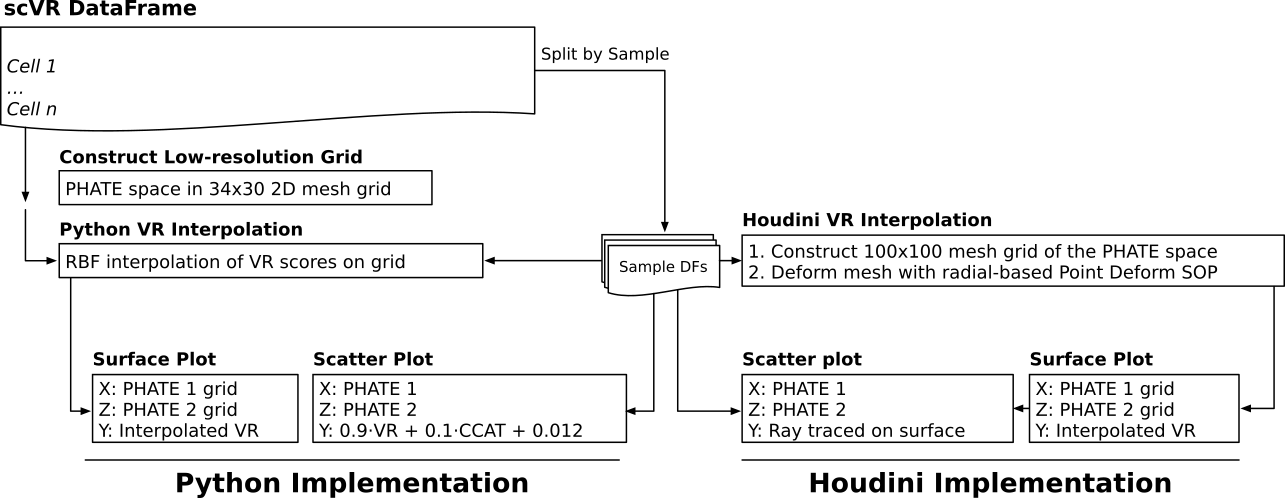
\includegraphics{02methods/figs/2VR_Landscape.png}
    \caption{}
    \label{}
\end{figure}

Finally, external software can also be used to render the data-driven landscapes, as shown in Qin \& Cardoso Rodriguez et al. 2023 where we used the 3D rendering programmes SideFX Houdini and Maxon Redshift.


% \subsection{Tool packaging/deployment with jupyter notebooks and nbdev}


% \colorbox{yellow}{Current notebook explanation}

% 1. Import necessary libraries: matplotlib, plotly, pandas, numpy, graphtools, scipy, sklearn
% 2. Define a function `compute_distdeg` that takes several arguments including an input dataframe, a column to split by, a list of columns to use for computation, and several optional arguments such as knn, distance metric, scale and plot options.
% 3. Within the `compute_distdeg` function:
%     a. Initialize an empty output dataframe with specified columns
%     b. Loop over unique values in the `split_by` column of the input dataframe
%     c. For each unique value:
%         i. Subset the input dataframe to only include rows where the `split_by` column equals the current unique value
%         ii. Create a graph using the subsetted dataframe and specified knn and distance metric
%         iii. Compute distances using shortest path on the graph
%         iv. Compute median distance to all cells for all cells
%         v. Add distance and degree columns to the subsetted dataframe
%         vi. Optionally remove outliers by replacing distant outliers with median value
%         vii. Optionally scale distance and degree columns
%         viii. Optionally plot cluster cells on phate and color by distance from centroid
%         ix. Concatenate subsetted dataframe with output dataframe
%     d. Return output dataframe
% 4. Load cell data from a csv file into a pandas DataFrame
% 5. Call `compute_distdeg` function on cell data with specified arguments and store result in a new DataFrame
% 6. Merge result with original cell data DataFrame on specified columns
% 7. Scale velocity length for all cells in cell data DataFrame using MinMaxScaler from sklearn.
% 8. Display final cell data DataFrame.


\section{Knowledge Graphs for Cell Communications}

\subsection{Sources and Assembly}

Assembling custom LRT:
Grab ligands and receptors from cellchat and nichenet LR interaction databses. ALso grab targets from nichenet database.
Targets subset so that there is no overlap with possible lignads and receptors.
To assemble the KG, iterate through all possible tail anad head pairs and then create a triplet if both belong to the same pathways in reactome (pathways of a poarticular level).
This pathway information gets encoded int he relation field.

Strtcutere: Nodes are genes and edges are "pathways".

\colorbox{yellow}{TABLE COMPARING BOTH KGs USED}

Assembling omnipath JG: \cite{turei_integrated_2021}
Omnipath has a curated functional interactions interaction database comprising genes involved in cellular communications. type of interactions (PTM, ...) consensus, directionality and even logical sense of interaction (activation or repression). HTis datasbase is cureated from public resources.
Grab the directed interactions and then add them to the head and tail of rthe KG. Relation field is computed ina  similar manner as the custom LRT using REactome pathway database.e


\subsection{KG Embedding}

Now with the triples assembled we can embedd our KG using pykeen \cite{ali_pykeen_2021}

Severela KGE modells available in pykeen. USed TranR \cite{lin_learning_2015} as it is an improved verion of the classical transE \cite{bordes_translating_2013} thatbetter encodes relations information. 

Embedding space is 50 dimensional and should caputre directional information and and relational info too (type of interactions between two ndoes).
Both nodes and edges can be embeeded using transR. 
Looking at nodes thsi means thatwe can see which kind of genes (lignas, receptors, targets,...) are present and how they dsitribute. WE can also check out the different pathawys they belong to and see if there is come kind of biologically driver distribution here re pathways.
Edges can also be embedded and hopefully lowere level pthawys belonging to a shared bigger levl pathways might lie in closer together? Also deppening on the ratio of shared interactions members between disticnt pathways. 
This can be benchamarked



\subsection{Wavelet Transform and Data Projection}

NOw, t difuees signals on the KGE graphs we used a wavelet transofrm approach.

The KGE space is now used to build a knn graphs on to wich the wavelets will be computed. For each of the nodes (genes) of the grapha a wavelet is centeread at then difussed at different scales. This reaults ina  bank of wavelets that centers around each node. 
Now this matrix contianing the genes X wavelts  and then do dot porcudt with the count magtrix having cells X genes. The result matgrix relfects how the cells are projected ont he graph, being cells x wavelet.
It can thus be used to compute a PCA space from which we will compute a knn and phagte spaces. phate space si sused to visually look at embedding. knn is used as the baseline grpah onto which we compute distances between cells.
If we also compute distnaces on the kmnn grpaph derived from gene expression and then sumamrise the distnaces by computing the mean distance of cells from a particualr c;uster to other clusters then we are able to benchark approach.

Becnhamark by computing distances on genex scpae and on projected spaces. Cells that are comunicating should, even if they transcriptoomic profiles aren't very similar, fall closer in the projected space than in the genex space.


% \subsection*{Emebdding LR pairs to recovr info on fucntional communication}


% ALternative approach goes here. Run current notebook version and get results with out data so I can at least set on a draft method approach



\section{FAIR spirit and reproduceability}

Data and code are FAIR:

* Findable
* Accessible
* Interoperable
* Reusable

The code for CyGNAL can be found in the group’s GitHub repository at  https://github.com/TAPE-Lab/CyGNAL and remains under continued development. In addition to the main steps already presented, there are also a set of utility scripts that can be used for performing common dataset manipulations; such as downsampling, concatenation, and format conversion. In Sup. Figure 1 a detailed diagram depicting CyGNAL’s steps is shown.








% \lstset{frameround=fttt,language=Python,numbers=left,breaklines=true}

% Test the text. Now with \texttt{cobra.flux\textunderscore analysis}!

% \begin{spacing}{1.5}
% \begin{lstlisting}[caption={Pseudocode snippet for \texttt{1-data\textunderscore preprocess.py}}, breaklines=true,basewidth=6pt,frame=single,language=Python, numbers=left, prebreak=**, postbreak=**, label={lst:code}]
% def run_meteor(model_path, constraints_path, **options):
%   # Load in the model
% 	model = cobra.io.read_sbml_model(model_path)
%   # Load and apply the options
% 	options = options.get('options', None)
% 	model = options_setup.apply_options (model, constraints_path, options)
%   # FBA: Parsimonious FBA
% 	model_solution = meteor_functions.perform_fba(model)
%   # Load in categories for CBA from options
% 	categories = options["categories"]
% 	atpbiomass_reactions = categories['ATP']['biomass']
% 	atpburned_reactions = categories['ATP']['burned']
% 	atpwaste_reactions = categories['ATP']['waste'] 
% 	nadpbiomass_reactions = categories['NADP']['biomass']
% 	nadpwaste_reactions = categories['NADP']['waste'] 
%   # Perform CBA and populate categories
% 	ATP_produced,..., NADP_waste = meteor_functions.cofactor_assessment(
%                                     model_solution, model, atpbiomass_reactions,
%                                     atpburned_reactions, atpwaste_reactions, 
%                                     nadpbiomass_reactions, nadpwaste_reactions)
%   # Populate respective dictionaries for the frontend tables
% 	metabolites = metabolite_config.metabolite_dict(model)
% 	reactions = reaction_config.reaction_dict(model, model_solution)
% 	objective = options_setup.get_objective(model)
%   # Get minimum/maximum fluxes for building the metabolic network
% 	flux = max(list(map(abs, (model_solution.fluxes))))
%   # Properly format the outputs
% 	assessment = meteor_functions.assessment_output(ATP_produced, ATP_metabolism,
%                 ATP_burned, ATP_biomass, ATP_waste, NADP_produced,
%                 NADP_metabolism, NADP_biomass, NADP_waste)
% 	result_categories = meteor_functions.category_dict(model, model_solution,
%                         atpwaste_reactions, ATP_waste, nadpwaste_reactions,
%                         NADP_waste, atpbiomass_reactions, atpburned_reactions,
%                         nadpbiomass_reactions)
% 	return metabolites, reactions, assessment, flux, model, result_categories, objective
% \end{lstlisting} 
% \end{spacing}



